\documentclass{standalone}
\usepackage{tikz}
\usetikzlibrary{patterns, positioning}

\begin{document}
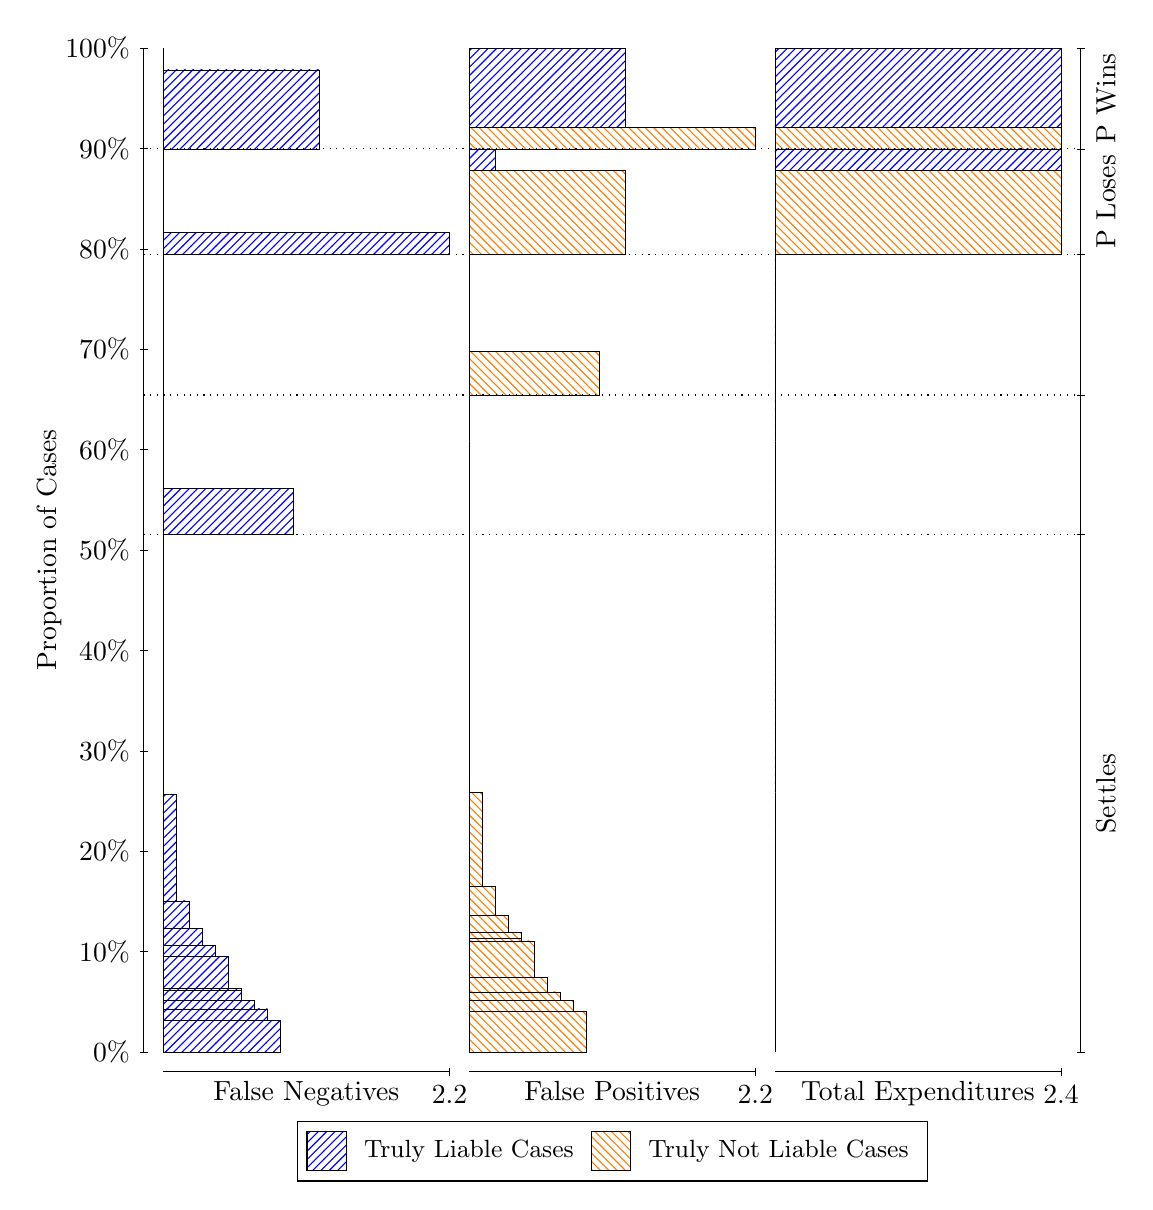
\begin{tikzpicture}
\draw[black, very thin] (1.5,1.75) -- (1.5,14.5);
\node[rotate=90, anchor=center] at (0.3, 8.125) {Proportion of Cases};
\draw[black, very thin] (1.45,1.75) -- (1.55,1.75);
\node[anchor=east] at (1.45, 1.75) {0\%};
\draw[black, very thin] (1.45,3.025) -- (1.55,3.025);
\node[anchor=east] at (1.45, 3.025) {10\%};
\draw[black, very thin] (1.45,4.3) -- (1.55,4.3);
\node[anchor=east] at (1.45, 4.3) {20\%};
\draw[black, very thin] (1.45,5.575) -- (1.55,5.575);
\node[anchor=east] at (1.45, 5.575) {30\%};
\draw[black, very thin] (1.45,6.85) -- (1.55,6.85);
\node[anchor=east] at (1.45, 6.85) {40\%};
\draw[black, very thin] (1.45,8.125) -- (1.55,8.125);
\node[anchor=east] at (1.45, 8.125) {50\%};
\draw[black, very thin] (1.45,9.4) -- (1.55,9.4);
\node[anchor=east] at (1.45, 9.4) {60\%};
\draw[black, very thin] (1.45,10.675) -- (1.55,10.675);
\node[anchor=east] at (1.45, 10.675) {70\%};
\draw[black, very thin] (1.45,11.95) -- (1.55,11.95);
\node[anchor=east] at (1.45, 11.95) {80\%};
\draw[black, very thin] (1.45,13.225) -- (1.55,13.225);
\node[anchor=east] at (1.45, 13.225) {90\%};
\draw[black, very thin] (1.45,14.5) -- (1.55,14.5);
\node[anchor=east] at (1.45, 14.5) {100\%};

\draw[black, very thin] (13.4,1.75) -- (13.4,14.5);
\draw[black, very thin] (13.35,1.75) -- (13.45,1.75);
\node[anchor=west] at (13.35, 1.75) {};
\draw[black, very thin] (13.35,8.3189) -- (13.45,8.3189);
\node[anchor=west] at (13.35, 8.3189) {};
\draw[black, very thin] (13.35,10.094) -- (13.45,10.094);
\node[anchor=west] at (13.35, 10.094) {};
\draw[black, very thin] (13.35,11.88) -- (13.45,11.88);
\node[anchor=west] at (13.35, 11.88) {};
\draw[black, very thin] (13.35,13.219) -- (13.45,13.219);
\node[anchor=west] at (13.35, 13.219) {};
\draw[black, very thin] (13.35,14.5) -- (13.45,14.5);
\node[anchor=west] at (13.35, 14.5) {};

\draw[black, very thin, pattern color=blue, pattern=north east lines] (1.75,1.75) rectangle (3.2364,2.1548);
\draw[black, very thin, pattern color=blue, pattern=north east lines] (1.75,2.1548) rectangle (3.0712,2.2972);
\draw[black, very thin, pattern color=blue, pattern=north east lines] (1.75,2.2972) rectangle (2.9061,2.4082);
\draw[black, very thin, pattern color=blue, pattern=north east lines] (1.75,2.4082) rectangle (2.7409,2.5342);
\draw[black, very thin, pattern color=blue, pattern=north east lines] (1.75,2.5342) rectangle (2.7409,2.5543);
\draw[black, very thin, pattern color=blue, pattern=north east lines] (1.75,2.5543) rectangle (2.5758,2.9687);
\draw[black, very thin, pattern color=blue, pattern=north east lines] (1.75,2.9687) rectangle (2.4106,3.1028);
\draw[black, very thin, pattern color=blue, pattern=north east lines] (1.75,3.1028) rectangle (2.2455,3.315);
\draw[black, very thin, pattern color=blue, pattern=north east lines] (1.75,3.315) rectangle (2.0803,3.6694);
\draw[black, very thin, pattern color=blue, pattern=north east lines] (1.75,3.6694) rectangle (1.9152,5.0218);
\draw[black, very thin, pattern color=orange, pattern=north west lines] (1.75,5.0218) rectangle (1.75,8.3189);
\draw[black, very thin, pattern color=blue, pattern=north east lines] (1.75,8.3189) rectangle (3.4015,8.912);
\draw[black, very thin, pattern color=orange, pattern=north west lines] (1.75,8.912) rectangle (1.75,10.094);
\draw[black, very thin, pattern color=orange, pattern=north west lines] (1.75,10.094) rectangle (1.75,10.651);
\draw[black, very thin, pattern color=blue, pattern=north east lines] (1.75,10.651) rectangle (1.75,11.88);
\draw[black, very thin, pattern color=blue, pattern=north east lines] (1.75,11.88) rectangle (5.3833,12.157);
\draw[black, very thin, pattern color=orange, pattern=north west lines] (1.75,12.157) rectangle (1.75,13.219);
\draw[black, very thin, pattern color=blue, pattern=north east lines] (1.75,13.219) rectangle (3.7318,14.223);
\draw[black, very thin, pattern color=orange, pattern=north west lines] (1.75,14.223) rectangle (1.75,14.5);
\draw[black, very thin, pattern color=orange, pattern=north west lines] (5.6333,1.75) rectangle (7.1197,2.2635);
\draw[black, very thin, pattern color=orange, pattern=north west lines] (5.6333,2.2635) rectangle (6.9545,2.4051);
\draw[black, very thin, pattern color=orange, pattern=north west lines] (5.6333,2.4051) rectangle (6.7894,2.5141);
\draw[black, very thin, pattern color=orange, pattern=north west lines] (5.6333,2.5141) rectangle (6.6242,2.6999);
\draw[black, very thin, pattern color=orange, pattern=north west lines] (5.6333,2.6999) rectangle (6.4591,3.1605);
\draw[black, very thin, pattern color=orange, pattern=north west lines] (5.6333,3.1605) rectangle (6.2939,3.1883);
\draw[black, very thin, pattern color=orange, pattern=north west lines] (5.6333,3.1883) rectangle (6.2939,3.2655);
\draw[black, very thin, pattern color=orange, pattern=north west lines] (5.6333,3.2655) rectangle (6.1288,3.4831);
\draw[black, very thin, pattern color=orange, pattern=north west lines] (5.6333,3.4831) rectangle (5.9636,3.8548);
\draw[black, very thin, pattern color=orange, pattern=north west lines] (5.6333,3.8548) rectangle (5.7985,5.0471);
\draw[black, very thin, pattern color=blue, pattern=north east lines] (5.6333,5.0471) rectangle (5.6333,8.3189);
\draw[black, very thin, pattern color=orange, pattern=north west lines] (5.6333,8.3189) rectangle (5.6333,9.5012);
\draw[black, very thin, pattern color=blue, pattern=north east lines] (5.6333,9.5012) rectangle (5.6333,10.094);
\draw[black, very thin, pattern color=orange, pattern=north west lines] (5.6333,10.094) rectangle (7.2848,10.651);
\draw[black, very thin, pattern color=blue, pattern=north east lines] (5.6333,10.651) rectangle (5.6333,11.88);
\draw[black, very thin, pattern color=orange, pattern=north west lines] (5.6333,11.88) rectangle (7.6152,12.943);
\draw[black, very thin, pattern color=blue, pattern=north east lines] (5.6333,12.943) rectangle (5.9636,13.219);
\draw[black, very thin, pattern color=orange, pattern=north west lines] (5.6333,13.219) rectangle (9.2667,13.496);
\draw[black, very thin, pattern color=blue, pattern=north east lines] (5.6333,13.496) rectangle (7.6152,14.5);
\draw[black, very thin, pattern color=orange, pattern=north west lines] (9.5167,1.75) rectangle (9.5167,5.0471);
\draw[black, very thin, pattern color=blue, pattern=north east lines] (9.5167,5.0471) rectangle (9.5167,8.3189);
\draw[black, very thin, pattern color=orange, pattern=north west lines] (9.5167,8.3189) rectangle (9.5167,9.5012);
\draw[black, very thin, pattern color=blue, pattern=north east lines] (9.5167,9.5012) rectangle (9.5167,10.094);
\draw[black, very thin, pattern color=orange, pattern=north west lines] (9.5167,10.094) rectangle (9.5167,10.651);
\draw[black, very thin, pattern color=blue, pattern=north east lines] (9.5167,10.651) rectangle (9.5167,11.88);
\draw[black, very thin, pattern color=orange, pattern=north west lines] (9.5167,11.88) rectangle (13.15,12.943);
\draw[black, very thin, pattern color=blue, pattern=north east lines] (9.5167,12.943) rectangle (13.15,13.219);
\draw[black, very thin, pattern color=orange, pattern=north west lines] (9.5167,13.219) rectangle (13.15,13.496);
\draw[black, very thin, pattern color=blue, pattern=north east lines] (9.5167,13.496) rectangle (13.15,14.5);
\draw[black, dotted] (1.5,8.3189) -- (13.4,8.3189);
\draw[black, dotted] (1.5,10.094) -- (13.4,10.094);
\draw[black, dotted] (1.5,11.88) -- (13.4,11.88);
\draw[black, dotted] (1.5,13.219) -- (13.4,13.219);
\draw[black, very thin] (1.75,1.5) -- (5.3833,1.5);
\node[anchor=north] at (3.5667, 1.5) {False Negatives};
\draw[black, very thin] (5.3833,1.45) -- (5.3833,1.55);
\node[anchor=north] at (5.3833, 1.45) {2.2};

\draw[black, very thin] (5.6333,1.5) -- (9.2667,1.5);
\node[anchor=north] at (7.45, 1.5) {False Positives};
\draw[black, very thin] (9.2667,1.45) -- (9.2667,1.55);
\node[anchor=north] at (9.2667, 1.45) {2.2};

\draw[black, very thin] (9.5167,1.5) -- (13.15,1.5);
\node[anchor=north] at (11.333, 1.5) {Total Expenditures};
\draw[black, very thin] (13.15,1.45) -- (13.15,1.55);
\node[anchor=north] at (13.15, 1.45) {2.4};

\node[black, centered, rotate=90] at (13.72, 5.0344) {Settles};


\node[black, centered, rotate=90] at (13.72, 12.55) {P Loses};
\node[black, centered, rotate=90] at (13.72, 13.86) {P Wins};

\draw (7.449999999999999,1.5) node[draw=none] (baseCoordinate) {};
\begin{scope}[align=center]
        \matrix[scale=0.5, draw=black, below=0.5cm of baseCoordinate, nodes={draw}, column sep=0.1cm]{
            \node[rectangle, draw, minimum width=0.5cm, minimum height=0.5cm, pattern=north east lines, pattern color=blue] {}; &
            \node[draw=none, font=\small] (B) {Truly Liable Cases}; &
            \node[rectangle, draw, minimum width=0.5cm, minimum height=0.5cm, pattern=north west lines, pattern color=orange] {}; &
            \node[draw=none, font=\small] (B) {Truly Not Liable Cases}; \\
            };
\end{scope}

\end{tikzpicture}
\end{document}